\documentclass[11pt]{article}
\usepackage{geometry, titlesec}
\usepackage[parfill]{parskip}
\usepackage[italicdiff]{physics}
\usepackage{amsfonts, amsthm}
\usepackage[cm]{fullpage}
\usepackage{fancyhdr}
\usepackage{enumitem}
\usepackage{xcolor, soul}
\usepackage{graphicx}
\usepackage[export]{adjustbox}
\usepackage{siunitx}
%\allowdisplaybreaks

\renewcommand{\thesubsection}{\thesection.\alph{subsection}}
\setenumerate[1]{label={(\alph*)}}

\makeatletter
\renewcommand*\env@cases[1][1.2]{%
  \let\@ifnextchar\new@ifnextchar
  \left\lbrace
  \def\arraystretch{#1}%
  \array{@{}l@{\quad}l@{}}%
}
\makeatother
 
\renewcommand{\footrulewidth}{.2pt}
%\setlist[enumerate]{leftmargin=*}
\pagestyle{fancy}
\fancyhf{}
\lhead{Physics 132-B}
\chead{\textbf{Discussion 7 Problems}}
\rhead{A--De Discussion}
\setlength{\headheight}{11pt}
\setlength{\headsep}{11pt}
\setlength{\footskip}{24pt}
\lfoot{\today}
\rfoot{\thepage}

\titleformat{\subsection}[runin]{\normalfont\large\bfseries}{\thesubsection}{1em}{}
\newcommand{\refeq}[1]{(\ref{#1})}

\newcommand{\beq}{\begin{equation*}}
\newcommand{\eeq}{\end{equation*}}

\newcommand{\beqn}{\begin{equation}}
\newcommand{\eeqn}{\end{equation}}

\newcommand{\blg}{\begin{align*}}
\newcommand{\elg}{\end{align*}}


\newenvironment{statement}
{
%    \color{gray}
    \ignorespaces
}
{
%    \smallskip
}

\newenvironment{problem}
{
%    \color{darkgray}
    \ignorespaces
}

\newenvironment{solution}
{
    \paragraph{Solution.}
    \ignorespaces
}
{
    \bigskip
}

\newcommand{\qimplies}{\quad \implies \quad}


\begin{document}
	


\newcommand{\vF}{\vb{F}}
\newcommand{\vv}{\vb{v}}
\newcommand{\vB}{\vb{B}}

\paragraph{Question 27.1}
\begin{problem}
	Can a charged particle move through a magnetic field without experiencing any force?  If so, how?  If not, why not?
\end{problem}

\vfill

\paragraph{Question 27.7}
\begin{problem}
	If the magnetic force does no work on a charged particle, how can it have any effect on the particle's motion?  Are there other examples of forces that do no work but have a significant effect on a particle's motion?
\end{problem}

\vfill

\paragraph{Question 28.4}
\begin{problem}
	Two parallel conductors carrying current in the same direction attract each other.  If they are permitted to move toward each other, the forces of attraction do work.  From where does the energy come?  Does this contradict the assertion in Chapter 27 that magnetic forces on moving charges do no work?  Explain.
\end{problem}

\vfill
%\clearpage

\paragraph{Question 28.10}
\begin{problem}
	What are the relative advantages and disadvantages of Ampere's law and the law of Biot and Savart for practical calculations of magnetic fields?
\end{problem}

\vfill

\clearpage


\newcommand{\tht}{\theta}
\newcommand{\muo}{\mu_0}
\newcommand{\lam}{\lambda}
\newcommand{\vL}{\vb{L}}

\begin{minipage}[l]{0.65\textwidth}
\paragraph{Problem 28.61}
\begin{problem}
	Two long, parallel wires hang by a \SI{4.00}{\cm}-long cords from a common axis~(\textbf{Fig.~P28.61}).  The wires have a mass per unit length of \SI{0.0125}{\kg\per\meter} and carry the same current in opposite directions.  What is the current in each wire if the cords hang at an angle of \SI{6.00}{\degree} with the vertical?
\end{problem}
\end{minipage}%
\hspace{0.05\textwidth}%
\begin{minipage}{0.30\textwidth}
\center 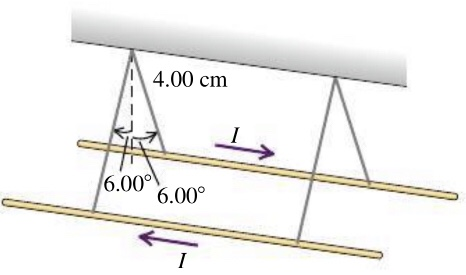
\includegraphics[width=\textwidth]{P28-61.jpeg}
\center \textbf{Figure P28.61}
\end{minipage}

\vfill 

\end{document}